\documentclass[a4paper,10pt,twoside,openright]{memoir}
\semiisopage
\checkandfixthelayout

\usepackage[T1]{fontenc}
\usepackage[utf8]{inputenc}
\usepackage{lmodern}

\usepackage{array,booktabs,mdwlist}
\renewcommand*{\arraystretch}{1.2}

\usepackage{amsmath,amssymb,amsthm,mathtools,relsize,stackengine}

\newcommand*{\PN}{\textnormal{\emph{PN}}}
\newcommand*{\LN}{\textnormal{\emph{LN}}}
\newcommand*{\HN}{\textnormal{\emph{HN}}}
\newcommand*{\EN}{\textnormal{\emph{EN}}}
\newcommand*{\PI}{\textnormal{\emph{PI}}}
\newcommand*{\xto}{}\let\xto\xrightarrow
\newcommand*{\vecarrow}{}\let\vecarrow\vec
\renewcommand*{\vec}[1]{\boldsymbol{\mathrm{#1}}}
\newcommand*{\EffC}[1]{\mathop{\textnormal{EC}\mathnormal{(#1)}}}
\DeclareMathOperator{\EME}{EME}
\DeclareMathOperator{\SME}{SME}
\DeclareMathOperator{\PriME}{\Pi ME}
\DeclareMathOperator{\HME}{HME}
\DeclareMathOperator{\MME}{MME}
\newcommand*{\MInv}[1]{\tau\vec{#1}}
\DeclareMathOperator{\StrC}{SC}
\DeclareMathOperator{\CasC}{CC}
\DeclareMathOperator{\SCC}{SCC}
\newcommand*{\CCS}{\textnormal{\emph{CCS}}}
\newcommand*{\ECS}{\textnormal{\emph{ECS}}}
\newcommand*{\TRS}{\textnormal{\emph{TRS}}}
\DeclareMathOperator{\diag}{diag}

\usepackage{xparse}

\usepackage{microtype}

\usepackage{tikz}
\usetikzlibrary{arrows,calc,positioning,shapes,matrix}
\usepackage[compactlambda]{petriTikz}

\pgfdeclarelayer{bg}
\pgfdeclarelayer{connections}
\pgfsetlayers{bg,connections,main}

\tikzset{>=latex'}

\newsubfloat{figure}

\usepackage[
  hyperfootnotes=false,
  breaklinks=true,
  hypertexnames=true,
  plainpages=false,
  pdfpagelabels=true,
  hidelinks
]{hyperref}

\usepackage[
  style=authoryear-comp,
  maxnames=2,
  maxbibnames=99,
  uniquename=init,
  uniquelist=false,
  backref=false,
  doi=false,
  isbn=false,
  eprint=false,
  natbib=true,
  hyperref=true,
  autolang=hyphen,
  backend=biber
]{biblatex}
\bibliography{markov}
\AtEveryBibitem{% Clean up the bibtex rather than editing it
  \clearlist{address}
  \clearfield{date}
  \clearfield{issn}
  \clearlist{location}
  \clearfield{month}
  \clearfield{series}
  \ifentrytype{book}{}{% Remove publisher and editor except for books
    \ifentrytype{inbook}{}{
      \clearlist{publisher}
      \clearname{editor}
    }
  }
  \ifentrytype{article}{
    \clearfield{url}}{}
  \ifentrytype{inproceedings}{
    \clearfield{url}}{}
}
\DefineBibliographyStrings{english}{%
  bibliography = {References}
}

\begin{document}

\mainmatter

\chapter{Example Petri Net}

We will now consider the Generalized Stochastic Petri Net $\PN$ in
Figure~\ref{fig:example:pn}~(a). The net contains seven places, two
immediate transitions $t_1$ and $t_3$, which form an effective
conflict set, and six timed transitions.

\begin{figure}
  \hspace*{\fill}
  \parbox[c]{0.55\linewidth}{\centering \begin{tikzpicture}
  \petriP(p1)(0,0){$p_1$}<1>
  \petriT(t1)(2,-0.8){$t_1$}<1>{2}
  \petriT(t2)(-2,-0.8){$t_2$}<1>{1}
  \petriP(p2)(3,-1.5){$p_2$}
  \petriP(p4)(1,-2.4){$p_4$}
  \petriT(t3)(0,-2.4){$t_3$}{1}
  \petriP(p5)(-1,-1.5){$p_5$}<1>
  \petriP(p3)(-3,-1.5){$p_3$}
  \petriT(t4)(2,-2.4){$t_4$}{0.1}
  \petriT(t5)(-2,-2.4){$t_5$}{0.1}
  \petriP(p6)(1,-4.3){$p_6$}
  \petriT(t6)(0,-4.3){$t_6$}{1}
  \petriP(p7)(-1,-4.3){$p_7$}
  \petriT(t7)(-2,-4.3){$t_7$}{2}

  \begin{pgfonlayer}{connections}
    \draw [->]
    (p1) edge (t1)
    (p5) edge (t1)
    (t1) edge (p2)
    (p1) edge (t2)
    (p5) edge (t2)
    (t2) edge (p3)
    (p4) edge (t3)
    (t3) edge (p5)
    (p2) edge (t4)
    (t4) edge (p4)
    (t4) edge (p6)
    (p3) edge (t5)
    (t5) edge (p5)
    (t5) edge (p7)
    (p6) edge (t6)
    (t6) edge (p7)
    (p7) edge (t7)
    (t7) to ++(-1.5,0) |- (p1);
  \end{pgfonlayer}

  \begin{pgfonlayer}{bg}
    \path [rounded corners=5pt,fill=black!10,draw,dashed]
    (-3.8,0.9) rectangle (3.5,-3.2);
    \path [rounded corners=5pt,fill=black!10,draw,dashed]
    (-2.5,-3.4) rectangle (2.5,-5.1);
    \node [anchor=north east] at (3.5,0.9) {$\LN_1$};
    \node [anchor=north east] at (2.5,-3.4) {$\LN_2$};
  \end{pgfonlayer}
\end{tikzpicture}}
  \hfill
  \parbox[c]{0.4\linewidth}{\centering \begin{tikzpicture}
  \petriP(pi1)(0,0){$\PI_1$}<1>
  \petriT(t4)(1.5,-1){$t_4$}
  \petriT(t5)(-1.5,-1){$t_5$}
  \petriP(pi2)(0,-2){$\PI_2$}
  \petriT(t7)(-1.5,-3){$t_7$}

  \begin{pgfonlayer}{connections}
    \draw [->]
    (pi1) edge (t4)
    (t4) edge (pi2)
    (pi1) edge (t5)
    (t5) edge (pi2)
    (pi2) edge (t7)
    (t7) to ++(-0.5,0) |- (pi1);
  \end{pgfonlayer}
\end{tikzpicture}}
  \hspace*{\fill}
  \par\vspace{0.5\onelineskip}
  \hspace*{\fill}
  \parbox[t]{0.55\linewidth}{\subcaption{%
      Partition consisting of regions $\LN_1$ and $\LN_2$}}
  \hfill
  \parbox[t]{0.4\linewidth}{\subcaption{High level structure}}
  \hspace*{\fill}
  \caption{Example Generalized Stochastic Petri Net $\PN$ with its
    initial marking $M_0$}
  \label{fig:example:pn}
\end{figure}

\section{Decomposition into High Level and Low Level Nets}

\subsection{Partitioning Into Minimal Regions}

To facilitate Kronecker analysis we partition the net into
\emph{minimal regions} following
\citet{DBLP:journals/sigmetrics/BuchholzK98}.

A set of transitions $T_r \subset T$ defines a region if
$({}^{\bullet, \circ}T_r)^{\bullet, \circ} = T_r$, where
${}^{\bullet,\circ}T_r = {}^{\bullet}T_r \cup {}^{\circ}T_r$ is set of
places connected to transitions in $T_r$ by input or inhibitor edges,
and $P_r^{\bullet, \circ} = P_r^{\bullet} \cup P_r^{\circ}$ is the set
of transitions connected to places in $P_r$ by input or inhibitor
edges. In other words, the minimum regions partition the set of
transitions $T$ such that no place is shared by two transitions for
different regions as input on inhibitor.

We first partition $T$ into singleton sets $(\{p_i\})_{i = 1}^7$, then
iterate over the places. In the $i$th iteration, all the sets which
share $p_i$ as input (or inhibitor) are merged. We only need to merge
regions in iterations when $p_i$ has at least two adjacent input (or
inhibitor) edges.


\subsection{Merging Minimal Regions into Subnets}

The minimal region $\{t_1, t_2, t_3, t_4\}, \{t_5\}$ has immediate
output transitions $t_1$ and $t_2$ which must be turned into internal
transitions by region merging. Moreover, minimal regions $\{t_7\}$ and
$\{t_8\}$ contain no internal (timed) behaviour, therefore, they also
need to be merged. We merge them with each other in order to divide
$\PN$ into $J = 2$ low-level nets and $k = 3$ output transitions
between them.

Partitioning of the net is illustrated in
Table~\ref{tbl:example:partition}.

\begin{table}
  {\centering
    \begin{tabular}{@{}lll@{}}
      \toprule
      & Action & Regions \\
      \midrule
      & Initialize & $\{t_1\}, \{t_2\}, \{t_3\}, \{t_4\}, \{t_5\},
                     \{t_6\}, \{t_7\}, \{t_8\}$ \\[0.5em]
      $p_1$ & Merge $t_1, t_2, t_3, t_4$ & $\{t_1, t_2, t_3, t_4\}, \{t_5\},
                     \{t_6\}, \{t_7\}, \{t_8\}$ \\
      $p_2$ & & $\{t_1, t_2, t_3, t_4\}, \{t_5\},
                     \{t_6\}, \{t_7\}, \{t_8\}$ \\
      $p_3$ & & $\{t_1, t_2, t_3, t_4\}, \{t_5\},
                     \{t_6\}, \{t_7\}, \{t_8\}$ \\
      $p_4$ & $t_1, t_3$ ok & $\{t_1, t_2, t_3, t_4\}, \{t_5\},
                     \{t_6\}, \{t_7\}, \{t_8\}$ \\
      $p_5$ & $t_2, t_4$ ok & $\{t_1, t_2, t_3, t_4\}, \{t_5\},
                     \{t_6\}, \{t_7\}, \{t_8\}$ \\
      $p_6$ & & $\{t_1, t_2, t_3, t_4\}, \{t_5\},
                     \{t_6\}, \{t_7\}, \{t_8\}$ \\
      $p_7$ & & $\{t_1, t_2, t_3, t_4\}, \{t_5\},
                     \{t_6\}, \{t_7\}, \{t_8\}$ \\[0.5em]
      $t_1$ & Merge $t_1, t_5$ & $\{t_1, t_2, t_3, t_4, t_5\},
                     \{t_6\}, \{t_7\}, \{t_8\}$ \\
      $t_3$ & Merge $t_3, t_6$ & $\{t_1, t_2, t_3, t_4, t_5, t_6\},
                     \{t_7\}, \{t_8\}$ \\[0.5em]
      $t_7$ & Merge $t_7, t_8$ & $\LN_1 = \{t_1, t_2, t_3, t_4, t_5, t_6\},
                     \LN_2 = \{t_7, t_8\}$ \\
      \bottomrule
    \end{tabular}
    \par}
  \caption{Partitioning the set of transitions into regions}
  \label{tbl:example:partition}
\end{table}

\subsection{Partial Place Invariants and MSIPs}

We first compute the $P$-invariants of $\PN$:
\begin{itemize*}
\item $\{p_2, p_3, p_4, p_5\}$,
\item $\{p_1, p_2, p_3, p_6, p_7\}$.
\end{itemize*}
The $P$-invariants of $\LN_1$ with the output transitions removed:
\begin{itemize*}
\item $\PI_1 = \{p_1, p_2, p_3\}$,
\item $\{p_2, p_3, p_4, p_5\}$.
\end{itemize*}
The $P$-invariant of $\LN_2$ with the output transition removed:
\begin{itemize*}
\item $\PI_2 = \{p_6, p_7\}$.
\end{itemize*}

\emph{Partial} $P$-invariants are invariants of the low-level nets
which are not invariants of the full net. Therefore, both $\LN_1$ and
$\LN_2$ have only one partial invariants, $\PI_1$ and $\PI_2$,
respectively. These invariants correspond to MSIPs in the high level
net $\HN$ an the extended nets $\EN_1$ and $\EN_2$. The high-level net
is shown in Figure~\ref{fig:example:pn}~(b).

\section{High-level and Low-level TRS exploration}

Because both the high-level and low-level nets are $1$-bounded, we
will denote a marking by the set of places which have a token,
e.g.~$M_0 = \{p_1, p_5\}$ in the original net $\PN$ and $M_0 =
\{\PI_1\}$ in $\HN$.

The set of reachable high-level states (macro-markings) are
\begin{equation*}
  \TRS(\HN) = \{s^H_1 = \{\PI_1\}, s^H_2 = \{\PI_2\}\} \text.
\end{equation*}
When exploring the tangible state-spaces of the low-level nets, we
also note which high-level marking a given state corresponds to:
\begin{align*}
  \TRS(\LN_1) &= S^{(1)}_1 \cup S^{(1)}_2 \text, \\
  S^{(1)}_1 &= \{s^{(1)}_{1} = \{p_1, p_5\}, s^{(1)}_{2} = \{p_2\},
              s^{(1)}_{3} = \{p_3\}\} \text, \\
  S^{(2)}_2 &= \{s^{(1)}_{4} = \{p_4\}, s^{(1)}_{5} = \{p_5\}\} \text,
  \\
  \TRS(\LN_2) &= S^{(2)}_1 \cup S^{(2)}_2 \text, \\
  S^{(2)}_1 &= \{s^{(2)}_{1} = \emptyset\} \text, \\
  S^{(2)}_2 &= \{s^{(2)}_{2} = \{p_6\}, s^{(2)}_{3} = \{p_7\}\} \text.
\end{align*}

A na\"\i ve approximation of the state space of $\PN$ is $\TRS(\LN_1)
\times \TRS(\LN_2)$. However, this set of states contains many
markings unreachable from $M_0$.

We will analyse the behaviour of $\PN$ as a CTMC over the state space
$S' = S'_1 \cup S'_2 = S^{(1)}_1 \times S^{(2)}_1 \cup S^{(1)}_2
\times S^{(2)}_2\}$.
Observe that the the global state $(s^{(1)}_{5}, s^{(2)}_{2})$ is
unreachable, because in order have a token in $p_5$, transition $t_6$
must be fired, however, in order to have a token in $p_6$, transition
$t_5$ must be fired. The true state space of $\PN$ is
$S = S' \setminus \{(s^{(1)}_{5}, s^{(2)}_{2})\}$.

While the introduction of low-level state-space partitioning by MSIPs
reduced the size of $S'$ considerably, the resulting Markov chain is
still not irreducible; we have to work around unreachable marking. In
addition, the reduction of state-space size---which reduces storage
requirements of probability vectors---increased the complexity of the
rate matrix, as we will see in the next Section.

\section{Rate Matrix Generation}

We will find the rate matrix as a block matrix of $\lvert S^H \rvert
\times \lvert S^H \rvert$ block, plus a diagonal correction term:
\begin{gather}
  Q_O = \left( \begin{array}{@{}c|c@{}}
                 Q_O[1, 1] & Q_O[1, 2] \\
                 \hline Q_O[2, 1] & Q_O[2, 2]
       \end{array} \right) \text, \\
  Q_D = \diag(\vec{e}^T Q_O) \text, \\
  Q = Q_O + Q_D \text,
  \intertext{where the $\lvert S'_{x} \rvert \times \lvert S'_{y}
    \rvert$ matrix $Q_O[x, y]$ describes the rate of transitions from
    macro-marking $s^H_{x}$ to $s^H_{y}$ and is of the form:}
  Q_O[x, y] = \begin{cases}
    \displaystyle \bigoplus_{j = 1}^J Q^{(j)}_L[x, x] +
    \sum_{i = 1}^{k_{x, x}} \bigotimes_{j = 1}^{J} Q^{j}_k[x, x] & \text{if
      $x = y$,} \\
    \displaystyle
    \sum_{i = 1}^{k_{x, y}} \bigotimes_{j = 1}^{J} Q^{j}_k[x, y] & \text{if
      $x \ne y$.}
  \end{cases} \label{eq:example:QO}
\end{gather}

\emph{Is it true in the general case that $k_{x,x} = 0$? An output
  transition adds at least one token to a place in a \emph{foreign}
  region, therefore increases the value of at least one partial
  P-invariant of that region. Therefore, no output transition may
  leave the MSIPs unchanged.}

The $\lvert S^{(j)}_{x} \rvert \times \lvert S^{(j)}_{x} \rvert$
matrix $Q^{(j)}_L[x, x]$ describes the effects of inner transitions in
$\LN_j$ when the current macro-marking is $s^H_x$. The
$\lvert S^{(j)}_{x} \rvert \times \lvert S^{(j)}_{y} \rvert$ matrix
$Q^{(j)}_i[x, x]$ describes the effects in $\LN_j$ of the $i$th
transition (out of $k_{x, x}$) which takes $\HN$ from $s^H_x$ to
$s^H_y$.

The local transition matrices are
\begin{align}
  Q^{(1)}_L[1, 1] &= \begin{pmatrix}
    0 & 2 & 1 \\
    0 & 0 & 0 \\
    0 & 0 & 0
  \end{pmatrix} \text,
  & Q^{(2)}_L[1, 1] &= \begin{pmatrix}
    0
  \end{pmatrix} \text, \\
  Q^{(1)}_L[2, 2] &= \begin{pmatrix}
    0 & 0 \\
    0 & 0
  \end{pmatrix} \text, &
  Q^{(2)}_L[2, 2] &= \begin{pmatrix}
    0 & 1 \\
    0 & 0
  \end{pmatrix} \text.
\end{align}

There are no output transitions that leave the macro-marking
unchanged, therefore $k_{1, 1} = k_{2, 2} = 0$. The transitions $t_5$
and $t_6$ take $s^H_1$ to $s^H_2$, while transition $t_8$ takes
$s^H_2$ to $s^H_1$, therefore $k_{1, 2} = 2$ and $k_{2, 1} = 1$.

First we construct the matrices corresponding to output transitions
$t_5$. Note that we write $\lambda(t_5)$ ad $\lambda(t_6)$ in the
appropriate cells of $Q^{(1)}_1[1, 2]$ and $Q^{(1)}_2[1, 2]$ instead
of $1$ in order to avoid multiplication by $\lambda$ in
\eqref{eq:example:QO}.
\begin{align}
  Q^{(1)}_1[1, 2] &= \begin{pmatrix}
    0 & 0 \\
    0.1 & 0 \\
    0 & 0
  \end{pmatrix} \text, &
  Q^{(2)}_1[1, 2] &= \begin{pmatrix}
    1 & 0
  \end{pmatrix} \text, \\
  Q^{(1)}_2[1, 2] &= \begin{pmatrix}
    0 & 0 \\
    0 & 0 \\
    0 & 0.1
  \end{pmatrix} \text, &
  Q^{(2)}_2[1, 2] &= \begin{pmatrix}
    0 & 1
  \end{pmatrix} \text. \\
\end{align}

To construct the matrices corresponding to $t_8$, we must model the
immediate random behaviour of $\LN_1$ due to $t_1$ and $t_3$ in
$Q^{(1)}_1[2, 1]$:
\begin{align}
  Q^{(1)}_1[2, 1] &= \begin{pmatrix}
    0 & \frac{1}{3} & \frac{2}{3} \\
    1 & 0 & 0
  \end{pmatrix} \text, &
  Q^{(2)}_1[2, 1] &= \begin{pmatrix}
    0 \\
    0.5
  \end{pmatrix} \text.
\end{align}

The full $Q$ matrix is
\begin{equation}
  Q = \left( \begin{array}{@{}ccc|cccc@{}}
               * & 2 & 1 & 0 & 0 & 0 & 0 \\
               0 & * & 0 & 0.1 & 0 & 0 & 0 \\
               0 & 0 & * & 0 & 0 & 0 & 0.1 \\
               \hline
               0 & 0 & 0 & * & 1 & 0 & 0 \\
               0 & \frac{1}{6} & \frac{1}{3} & 0 & * & 0 & 0 \\
               0 & 0 & 0 & 0 & 0 & * & 1 \\
               0.5 & 0 & 0 & 0 & 0 & 0 & * \\
             \end{array} \right) \text.
\end{equation}
Observe that the second-to-last column contains no positive entries,
therefore, the corresponding $(s^{(1)}_5, s^{(2)}_2)$ state is indeed
unreachable and the CMTC is not irreducible.

\section{Kronecker Analysis with Decomposition}

\chapter{Kronecker Analysis}

\begin{figure}
  {\centering
    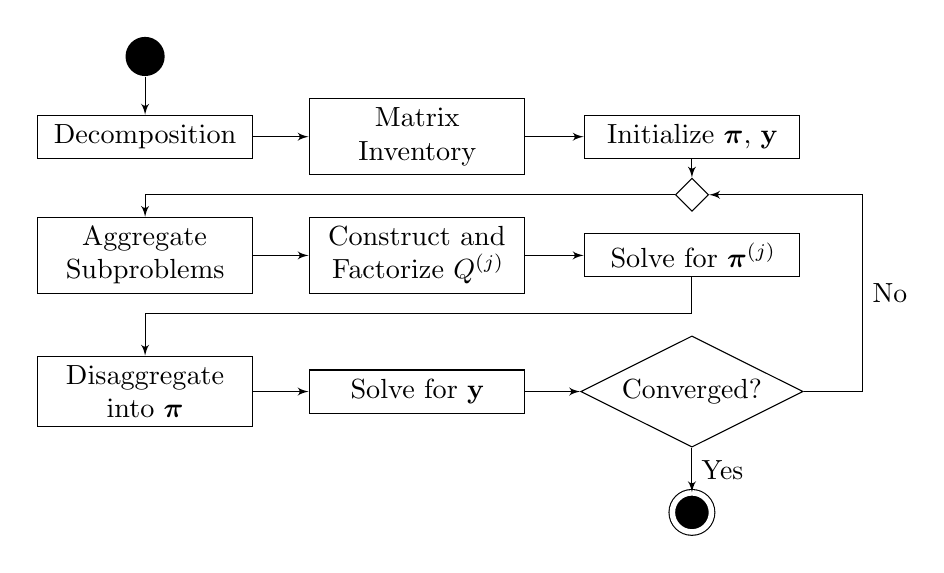
\begin{tikzpicture}[
  process/.style={
    text width=2.5cm,
    align=center,
    draw
  }
  ]
  \matrix [column sep=20pt,row sep=15pt] {
    \node (start) [fill=black,circle,inner sep=5pt] {}; \\[-7pt]
    \node (decompose) [process] {Decomposition}; &
    \node (matrix) [process] {Matrix\\Inventory}; &
    \node (init) [process] {Initialize $\vec{\pi}$, $\vec{y}$}; \\
    \node (aggregate) [process] {Aggregate\\Subproblems}; &
    \node (factorize) [process] {Construct and\\Factorize $Q^{(j)}$}; &
    \node (solve) [process] {Solve for $\vec{\pi}^{(j)}$}; \\
    \node (disaggregate) [process] {Disaggregate\\into
      $\vec{\pi}$}; &
    \node (correct) [process] {Solve for $\vec{y}$}; &
    \node (converged) [draw,diamond,aspect=2,inner sep=2pt]
    {Converged?}; \\
    & & \node (end) [draw,double,double distance=2pt,fill=black,circle,inner sep=5pt] {}; \\
  };
  \node (beforeaggregate) [diamond,inner sep=3pt,draw] at
  ($(init.south)+(0,-13pt)$) {};
  \draw [->] (start) edge (decompose);
  \draw [->] (decompose) edge (matrix);
  \draw [->] (matrix) edge (init);
  \draw [->] (init) edge (beforeaggregate);
  \draw [->] (beforeaggregate) -| (aggregate);
  \draw [->] (aggregate) edge (factorize);
  \draw [->] (factorize) edge (solve);
  \draw [->] (solve.south) to ++(0,-13pt) -| (disaggregate);
  \draw [->] (disaggregate) edge (correct);
  \draw [->] (correct) edge (converged);
  \draw [->] (converged.east) to ++(0.75cm,0) |- node [near
  start,right] {No} (beforeaggregate);
  \draw [->] (converged) edge node [right] {Yes} (end);
\end{tikzpicture}
    \par}
  \caption{The exact decompositional algorithm}
  \label{fig:kronecker:flowchart}
\end{figure}

Rough outline for figuring out the exact decomposition algorithm
\citep{bao2008decompositional} in Figure~\ref{fig:kronecker:flowchart}:

\section{Construction of Initial Probability Vector}

Due to the reducibility of $Q$, the initial choice of $\vec{\pi}$ will
determine the steady-state solution. Therefore, we need to choose
$\vec{\pi}$ such that it is only nonzero at the states reachable from
$M_0$,
\begin{equation}
  \pi_i = \begin{cases}
    1 / \lvert \TRS(\PN) \rvert & \text{if $s_i \in \TRS(\PN)$,} \\
    0 & \text{if $s_i \notin \TRS(\PN)$.} \\
  \end{cases}
\end{equation}
This requires discovery of $\TRS(\PN)$.

\section{Solution of the Reducible Subproblem}

Due to the block structure of $Q^{(j)}$, the ``projection'' of $Q$ to
$\LN_j$ which is obtained by removing the Kronecker products from
\eqref{eq:example:QO}, it is never irreducible. State changes which
would allow $Q^{(j)}$ to move between different macro-markings would violate
the partial $P$-invariants of $\LN_j$ which are used to describe the
macro-markings.

Therefore, we have to disaggregate and aggregate the synchronized part
of $Q$ in the decompositional algorithm. This reduces the
decompositional algorithm of \citet{bao2008decompositional} to the
approximate decompositional algorithm of
\citet{DBLP:journals/sigmetrics/BuchholzK98}, plus a Gauss--Seidel
correction step.

\section{Disaggregation of the Probability Vector}

After solving the local equations with (dis)aggregated synchronized
transitions, we obtain local probability vectors $\pi^{(j)}$ for each
local net $\LN_j$. Due to the reducibility of $Q$, the
vector Kronecker product
\begin{equation}
  \vec{pi}' = \bigotimes_{j = 1}^J \vec{\pi}^{(j)}
\end{equation}
cannot be used as input for the GS correction step, because it can
have support at states unreachable from $M_0$.

\section{Correction Vector Calculation}

(Block) Gauss--Seidel, as presented in the book, only works on sums of
Kronecker products, not block matrices where each block is a sum of
Kronecker products. Therefore, another method is needed to calculate
the correction vector $\vec{y}$.

Could (Block) Jacobi or (Block) power iteration \citep[Section
3.2]{dayar2012analyzing} be used here? Another possibility is a
``hybrid'' Jacobi--Gauss--Seidel approach, where we use Gauss--Seidel
backward substitution is used for the diagonal block, but the
off-diagonal blocks are zero in the matrix we need to ``invert'' in
matrix splitting.

\backmatter

\printbibliography

\end{document}